\documentclass[conference]{IEEEtran}
% If the IEEEtran.cls has not been installed into the LaTeX system files,
% manually specify the path to it. e.g.
% \documentclass[conference]{./IEEEtran}

% Add and required packages here
\usepackage{graphicx,times,amsmath, hyperref}

% Correct bad hyphenation here
\hyphenation{op-tical net-works semi-conduc-tor IEEEtran}

% To create the author's affliation portion using \thanks
\IEEEoverridecommandlockouts

\textwidth 178mm
\textheight 239mm
\oddsidemargin -7mm
\evensidemargin -7mm
\topmargin -6mm
\columnsep 5mm

\begin{document}

% Project title: keep the \ \\ \LARGE\bf in it to leave enough margin.
\title{\ \\ \LARGE\bf Open Streets Race}

\author{Anders Mousten, Michele Ermacora}

% Uncomment out the following line for invited papers
%\specialpapernotice{(Invited Paper)}

% Make the title area
\maketitle

%\begin{abstract}
%
%\end{abstract}

\section{Introduction}

Open Streets Race is a Unity \cite{unity} plug-in created for generation of tracks for racing games. The data is obtained from the Open Street Maps website \cite{openstreet}. Open Street Maps is a website similar to Google Maps \cite{gmaps} where the user can select different parts of the earth, but with an important difference: the user can also download parts of the maps obtaining informations about that zone (for example position of the roads, position of the buildings and size of them). This information can be downloaded as xml files, with nodes representing different objects (for example buildings, streets, parks, rivers, etc.). The goal of our plug-in is to let the user import the data into the Unity \cite{unity} engine in a simple way, and generate levels using real world cities data for a procedural content generation algorithm. These algorithms were developed such that the user can generate levels while maintaining control over the content generated. For this reason we have used different kinds of layers representing the different steps in generating a level; an example of this is the game play layer, where the user can decide to smooth the roads, place checkpoints and a car. This way, the generation of levels for car racing games becomes faster, while it gives the user control over the results. Another important aspect of our plug-in is that it is easy to include other kinds of constraints inside the game play layer, making it easy extendible, also for other kind sof genres (like FPS).

\section{Backgorund}

This work was inspired by the SketchaWorld system \cite{sketchaworld}. In this system the user can concentrate on what they want to create instead of how, by using a constraint solving system and semantic modelling. This is achieved by dividing the different parts of the level creation into different layers. For example, in the first layer (called landscape) the user can create the terrain, modify the height of it applying an height map or using the tools inside the editor. In the second (water), the user can create rivers. To do this, he can click on different parts of the maps and the PCG algorithm automatically generates the river, taking into consideration also the layer below, modifying it if necessary. In fact, in their framework, the layers above can modify the lower ones, using the constraints inside each of them to resolve the conflicts. The user can select to create a world from scratch, or import data from Open Street Maps and generate the world from there. \newline\newline
While this framework can generate very interesting worlds, with rivers, mountains, roads and cities that are fitting nicely together, one critique that can be done is that the, even though it was created for game developers, the developers have not added a game play layer (or taking into consideration the game play element). This causes the generation of realistic worlds, but it is not interesting from a game play perspective. For example, in an FPS set in a city background, we do not want only the generation of buildings, rivers, roads etc., but also covers, shortcuts between buildings, stairs that can make the players reach the roof and so on.
\newline
\newline
Another paper that inspired this work was Generating Interesting Monopoly Boards from Open Data \cite{monopoly}. In this paper the authors use Open World Data, taking into account the economic and social indicators from the UK government to generate the boards. This is done by using an evolving algorithm in which the different weights are evolved  for the street creation inside the Monopoly game. The user can decide which indicators to use for defining what means prosperity inside an area, and then, after some calculations, the board is generated. This paper is interesting as it uses real world data for generating Monopoly boards, letting the user create his own board based on his knowledge of what rich means, even though the main goal of this project was not the enjoyment of the player while playing on the board, as much as the thinking process on how to create it.
\newline
\newline
In 2001 Parish and Mueller \cite{parish} published a paper about how to procedurally generate large city areas based on geographical and sociostastistical maps. Examples here are elevation-, vegetation- and population density maps. Based on the image maps, road maps were created using an extended L-System that allowed an easy addition of new rules or subsystems (e.g. transportation networks). The roadmap was then used as a basis for subdivision into lots, which provided allotments for the building generation. Buildings were modelled by a parametric, stochastic L-System that used the footprint of the building (allotment) as the axiom. This enabled the L-System to improve the Level of Detail (LOD) of a building with each expansion, such that after one expansion the building was a simple extrusion, after two it could undergo the transformations of the production rule (scale, translate etc.) resulting in more and more submeshes of different dimensions and thereby an increase in detail.


\section{Game Design}

As said before, the main goal of our project is to give to the final user a tool for generating levels from real world data. To demonstrate how it could be applied to a game context, we focus on building a game play layer for a car racing game based on real world cities. The game play is inspired by other car racing games such as Need For Speed \cite{nfs}, in which the player can race inside a city in a free roaming way, and in which, inside the different race competitions, the user could also take advantage of the shortcuts (when present). Because modelling an entire real city (as Copenhagen) from scratch would require too much effort, we decided to create it using procedural content generation algorithms for generating the buildings and the roads from the data from Open Street Map. This way, we can also modify the different elements without having the need to re-create big models from scratch or modifying them. For example, instead of trying to make fit different shapes of curves, we need only to click where we want the road to start and end, and the algorithm takes care of generating the entire street (that can also be modified by the game play layer). Thus, having at our disposal this layer makes it more easy for us try different kinds of solutions for the track, improving the final quality of it.

\section{Methods}

In this section we are going to explain the different elements composing our plug-in.

\subsection{XML Parser}

The first element the user will use is the xml parser. This is a dll file in which the user can select which kind of data to import from the xml document downloaded from Open Street Maps. The dll supports the export of buildings, streets, rivers and parks. This is also easily extendable by overriding the parser method.
While in the start our idea was to implement a local database where to store the data from the xml files, we soon discovered that Unity was not capable of accessing it. We decided therefore to create a text file with the information that will be processed by the different layers implemented inside Unity. Because Open Street maps cannot export very big maps as xml files, the dll gives the possibility to also attach to the same text file nodes from different xml files, leaving to the user complete freedom on which zones (also coming from different places) he wants to use for his level creation, and how big the level should be.

\subsection{Building Layer}
After parsing the xml file, the sytem can generate buildings based upon the data from the parser. The user can specify if all the buildings should be built (default option) or only a subset. The user is also in control of the minimum and maximum height of the buildings. Each building is then assigned a random height within that interval. Prior to generating the buildings, the LSystem is initialized. Based on the production rule (editable by user) the axiom is expanded for a number of expansions. Then, for each building its lot coordinates are used as vertices for the footprint. These vertices are saved into the initial state of the building. As in a classic turtle-based LSystem, the "drawing" of the building is based on a stack, such that the symbols '[' and ']' respectively pushes the current state to the stack (saving) and assigns the current state to the state popped from the stack (loading). \newline

For each building, the expanded axiom is traversed. Normally, the first symbol is 'E', which marks an extrusion. A visualizer class provides functions for extrusion, scaling and translation. Extrusion is performed on the face of the current state. Initially, this is the footprint of the building. It works by taking a copy of the face vertices and translating them on the z-axis for the specified height. Then, it defines the triangles for vertical sides of the building, followed by the top of the building. It is not necessary to triangulate the bottom side since it will not be visible. Normals are computed my subtracting the position of each vertex with the mean center of all the vertices, and then normalizing the resulting vector. A new game object is added as a chilld to the game object of the current state. A mesh component that is assigned the found vertices, triangles and normals is added to the new game object, and the game object and its top face is assigned to the current state. The scaling function simply scales the game object's transform component and face vertices of the current state. Similarly, the translation function translates the transform and face coordinates.\newline

After visualization, a box collider is added to each building, along with a script that detects colliding roads. This allows for removal of buildings that are in the way of roads.

\subsection{Roads Generation}

For the road generation we decided to use an external plug-in \cite{plugin} to have the basic functionality of generating a mesh from a predefined set of points. For this script to be functional, it needs to be attached to a terrain. This gives the user the freedom of generating procedurally part of the background or modifying the terrain itself (as creating hills for example), as well as the roads, as the buildings automatically position themselves on top of the created terrain. This script simply takes as input a start and end position (created by the user by pointing the mouse cursor onto the point of the terrain in which he wants create the node while presses R), and. From these points, it searches inside the data structure storing all the real world streets and which nodes are most near to these points, and then it generates the street. As a search algorithm, we used A* , in which the heuristic function is the euclidean distance between the nodes  inside our data structure that the user has clicked on. After the real world road is found, we pass the nodes composing it to the external plug-in for the mesh generation. This plug-in applies a natural cubic spline \cite{spline} function to approximate the curve between the different nodes and create a smooth path.
If, between the points that the user has clicked, there is a hill, the algorithm also takes care of placing the different parts of the mesh on top of the terrain.

\subsection{Game Play Layer}

The game play layer is the last one that the user can interact with and represents a layer in which we modify the world created until now to fit the game play constraints that the designer wants to have. In this layer, for example, the user can select how to place the different checkpoints, a car and if he wants to smooth the path between particular points. \newline\newline
The smoothing road script applies the bezier curve function to smooth the path. This algorithm was chosen because it gives a certain degree of control, in which the user can select how many nodes to create during the smoothing process (the more nodes the user selects, the more smooth the path becomes). The bezier algorithm takes four points, called control points (P0,P1,P2,P3), in which the first and the last represent the start and the end of the curve, while the other two points represent how much the curve has to be tangent to the segment created by P0 - P1 and P2 - P3. The longer these two segments are, the more the resultant curve will tangent to them. When applying this method we pass to it the points that the user has clicked on (representing P1 and P2), plus the previous point of the first one selected (P0), and the one that follow the last point clicked on (P3). The algorithm also takes as a parameter the number of iterations it has to perform the path smoothing for (each iteration corresponds to a new node). The more iterations that are done, the more the smoother the path becomes. Finally, the points created, are passed to the road creation script (used in the Road Generation Layer) to create the new mesh.
The user can then decide which kind of road that fits better the level he has in mind.\newline\newline

The user can also add checkpoints. To do so, he presses D once, which spawns a checkpoint at the mouse cursor. Then, the user can move the checkpoint around using the mouse, and rotate it by holding down Shift while moving the mouse. The checkpoints allows the user to respawn the car from the latest checkpoint he drove through. This might be benefical if the car is off the track, or if possible, fatally damaged. This functionality was implemented by adding an empty spawn object to the checkpoint prefab that is placed exactly where we want the car to respawn relative to the checkpoint. An arrow texture was placed on a transparent plane beneath the checkpoint to show the user the right direction through the checkpoint. This was necessary because a new checkpoint was registrered by a trigger placed inside the checkpoint. If a user then drove through the checkpoint in the wrong direction, the car would respawn facing the checkpoint and result in a redundant save of the same checkpoint. To respawn a car, its transform was simply set to the transform of the spawning point of the latest checkpoint.

\section{Results}

The end results of our plug-in are quite interesting. The development of a car racing game is sped up quite a lot, as the user does not have to create meshes and can concentrate his efforts on improving the game play. Even the game play layer has decreased the time of development; in fact the end user can for example smooth the path and see different kind of solutions, only with the click of a button.\newline\newline
Also the results that we have using real world data were interesting.  In fact, they give the opportunity to generate real cities that have interesting patterns for generating arcade car racing games (for example Need For Speed). The opportunity to also use more than one kind of city for generating a single map, gives the freedom to the user to generate maps with different topologies that result in interesting worlds. Below follows some screenshots from the plugin that shows examples of generated buildings, roads, shortcuts, checkpoints and a car racing on one of the created tracks.

\begin{figure}[h!t]
\centering
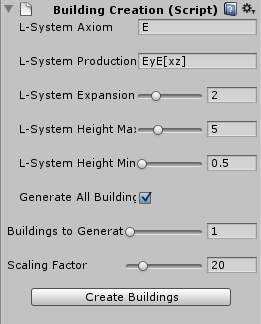
\includegraphics[scale=0.8]{images/BuildingScript.png}
\caption{\label{buildings} Screenshot of parameters that the user can specify when generating buildings}
\end{figure}

\begin{figure}[h!t]
\centering
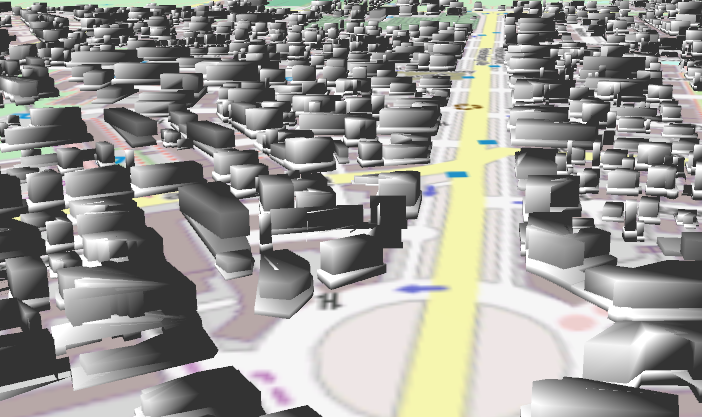
\includegraphics[scale=0.45]{images/Buildings4.png}
\caption{\label{buildings} Screenshot of generated buildings}
\end{figure}

\begin{figure}[h!t]
\centering
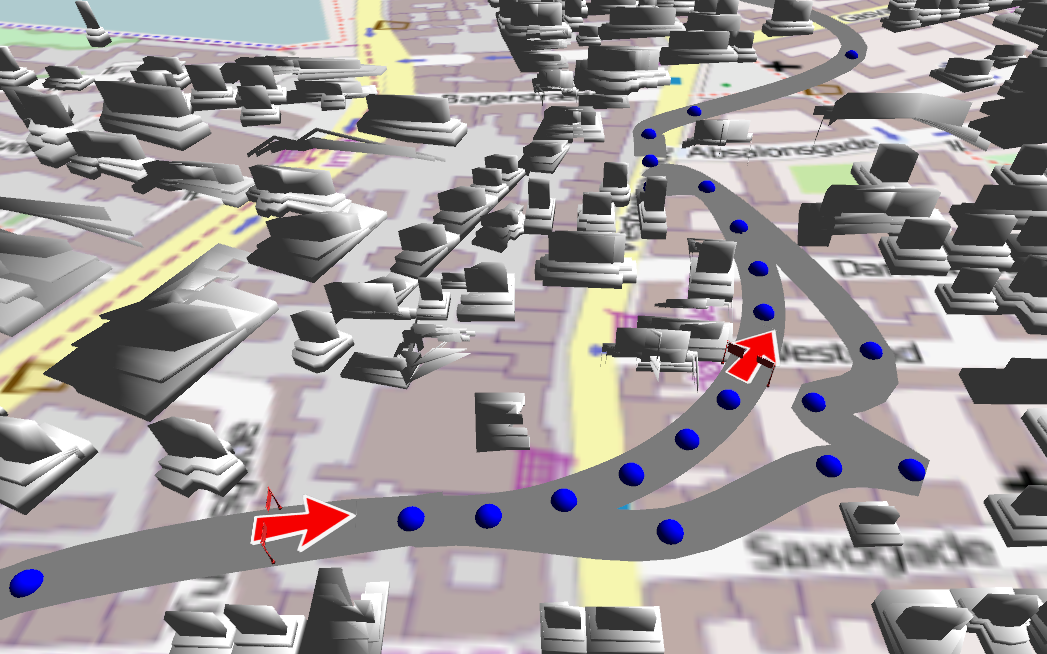
\includegraphics[scale=0.3]{images/Checkpoints1.png}
\caption{\label{buildings} Screenshot of a shortcut with checkpoints}
\end{figure}

\begin{figure}[h!t]
\centering
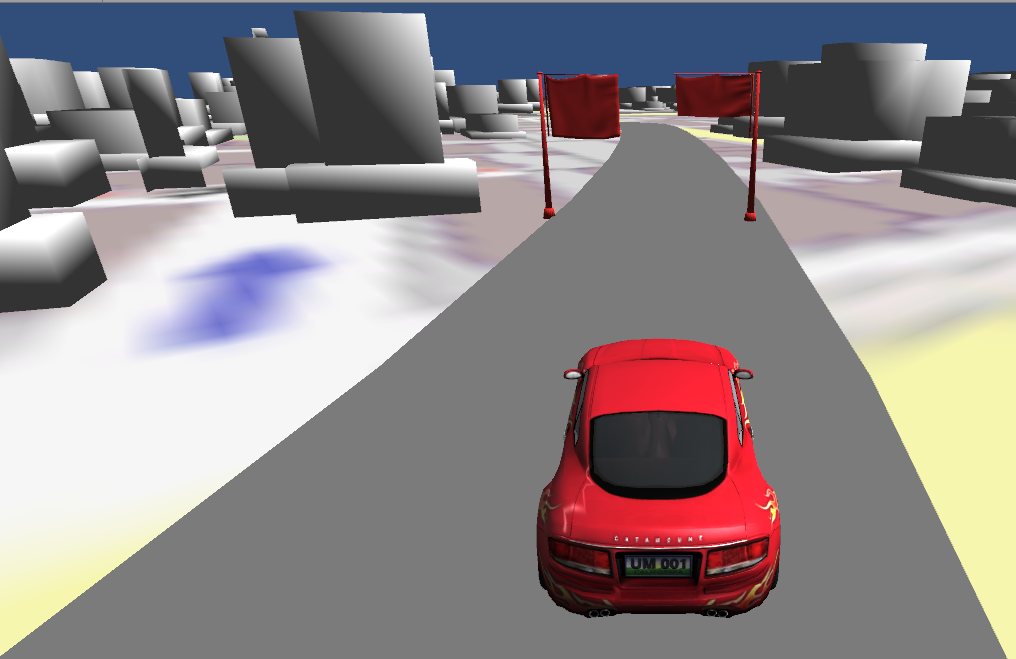
\includegraphics[scale=0.3]{images/Car1.png}
\caption{\label{buildings} Screenshot of ``in-game" driving}
\end{figure}

\subsection{Performance Analysis}

The most time consuming step is the building generation, that takes approximately 1 second for 100 buildings, so for a large city area with 3000 buildings, it takes around half a minute. This can be caused by the high number of instantiations of the game objects and mesh components, as well as the triangulation computations. The second most time consuming process is the parsing of the XML file, which takes around 3 seconds for a file with 40.000 nodes. The rest of the operations, such as road creation, shortcut placement and adding checkpoints takes a couple of hundred milliseconds at most.

\section{Discussion}

\subsection{Strengths}

Our plug-in has proved to have different kinds of strengths. One of them is the opportunity to use more than one kind of city for generating a single map, giving the freedom to the user to generate maps with different topologies that result in interesting worlds. Also, the time invested by generating a basic, playable level, is decreased largely thanks to automatic generation of buildings and streets. An other good point of our system is that, leaving to the player control over the generation algorithms, gives him the possibility to generate almost exactly what he wants. A final point to take into consideration is the extremely modularity of the game play layer, due to the presence of this plug-in inside the Unity engine. In fact, thanks to these two elements, the plug-in could be extended, very easily, to fit every kind of game genre. 

\subsection{Improvements}

While the end results was interesting, there is still room for improvements inside our plug-in.

\subsubsection{XML Parser}

The xml parser could be improved by the use of a database, which generates and uses text files, for accessing the information of the different nodes in a faster, more efficient and customizable way. In fact, using a SQL database, gives the user the freedom to generate tables in an easy way and then use his own customized tables.

\subsubsection{Buildings}
Now, The buildings are essientally generated by extruding their footprints and performing a sequence of transformation (scaling and translation). An improvement could be analyse the different nodes composing a building and use an appropriate shape (for example a cylinder for a round building, a cube for a skyscraber). This would simplify their visual look, but significantly decrease the creation time. One could then compensate for the low mesh detail by adding textures to the buildings. One approach would be to make the a pool of textures offline, and then select one randomly for each building. The selection could also depend on the dimensions of the buildings or parameters specified by the user. Another possibility would be to generate the textures procedurally, for instance using a grammar algorithm. An other improvement could also generate buildings that have actually interiors, (like for examples different floors, stairs, ecc). While for a car racing game this is not important, for a FPS this can increase the immersion of the player. \newline\newline
Currently, buildings that are in the way of roads are destroyed. It would, however, be interesting to apply boolean mesh operations to the colliding meshes. Instead of completely removing a building, one could subtract the road mesh from the building mesh, such that the resulting building would have a tunnel carved through it. Then various parameters could control the properties of such tunnels, e.g. dimensions and light properties.\newline\newline
 On some of the buildings, there were some glitches caused by overlapping triangles defined in the extrusion function. This is caused by convex building lots. As it works now, all the triangles of the top face are drawn from the first vertex to each pair of subsequent vertices. This could be solved by developing a more sophisticated triangulation algorithm, that changes the starting corner of some of the triangles based on trigonometric calculations of the vertex positions. 

\subsubsection{Roads}

Also the generation of roads can be improved. In fact, the generation of the mesh, while now is done in a single thread, could be better if it could be done in multi thread (feature not supported by Unity right now). Also, the smoothing of the path could be improved by implementing different textures (depending on the type of street) and new elements (like lights, lamps ecc.). Another improvement could be to select different kinds of algorithms depending on the degree of smoothing the user wants. Right now, it is not possible to create sharp corners.

\subsubsection{Gameplay Layer}

Finally, the game play layer can be improved by including more constraints, as, for example constraints regarding more cars driving at the same time (an example of constraint can be the size of the road depending of the number of cars playing the game). A weather system with different kinds of weather effects could also influence the gameplay, for instance rain could cause slippery roads. In general, more road types would increase the variety of the created racing tracks. For arcade racing, it might be fun to add turbo segments that accelerate the car, jumps etc.

\subsection{Additional Future Perspectives}
Another improvement can be done by implementing different kind of elements, instead of only buildings and roads, like trees, lakes, rivers ecc.

\begin{thebibliography}{6}
\bibitem{unity} Unity, Unity Technologies, http://unity3d.com/

\bibitem{openstreet} Open Street Maps, licensed under the Creative Commons Attribution-ShareAlike 2.0, http://www.openstreetmap.org/

\bibitem{gmaps} Google Maps, http://maps.google.com/

\bibitem{parish} Parish, Müller, ``Procedural Modeling of Cities", Siggraph, 2001.

\bibitem{sketchaworld}
Smelik, Tutenel, et al. ``A declarative approach to procedural modeling of virtual worlds" in \emph{Computers \& Graphics}, 2011, pp. 352-363.

\bibitem{monopoly} Gustafsson, Togelius. ``Generating Interesting Monopoly Boards from Open Data", 2012.

\bibitem{nfs} Need for Speed, EA Canada et. al, Electronic Arts, 1994-2012.

\bibitem{plugin} Chris Morris, ``Road/Path Tool",  Six Times Nothing, 2010.

\bibitem{spline} Patch Kessler, ``Natural Cubic Spline Interpolation", February 23, 2006.


\end{thebibliography}

% That's all folks...
\end{document}
